\documentclass[../main.tex]{subfiles}

\begin{document}

\section{Approach overwiew}
\label{section:lauxus:approach}
\par After all the previous introduction sections, we can start to explain the solution we designed to address the problem. In this section, we will explain the solution at a high level. Figures \ref{figure:lauxus:approach_trust} to \ref{figure:lauxus:approach_crypto} present this protocol and will be the heart of this section. Detailed insights will be discussed in Chapter \ref{chapter:lauxus}. The approach will be split into four parts for ease of understanding each major point of the protocol. The whole protocol is also presented at the end of this section.


\subsection{Trust overview}
\label{section:lauxus:approach_trust}
\begin{figure}[h]
    \centering
    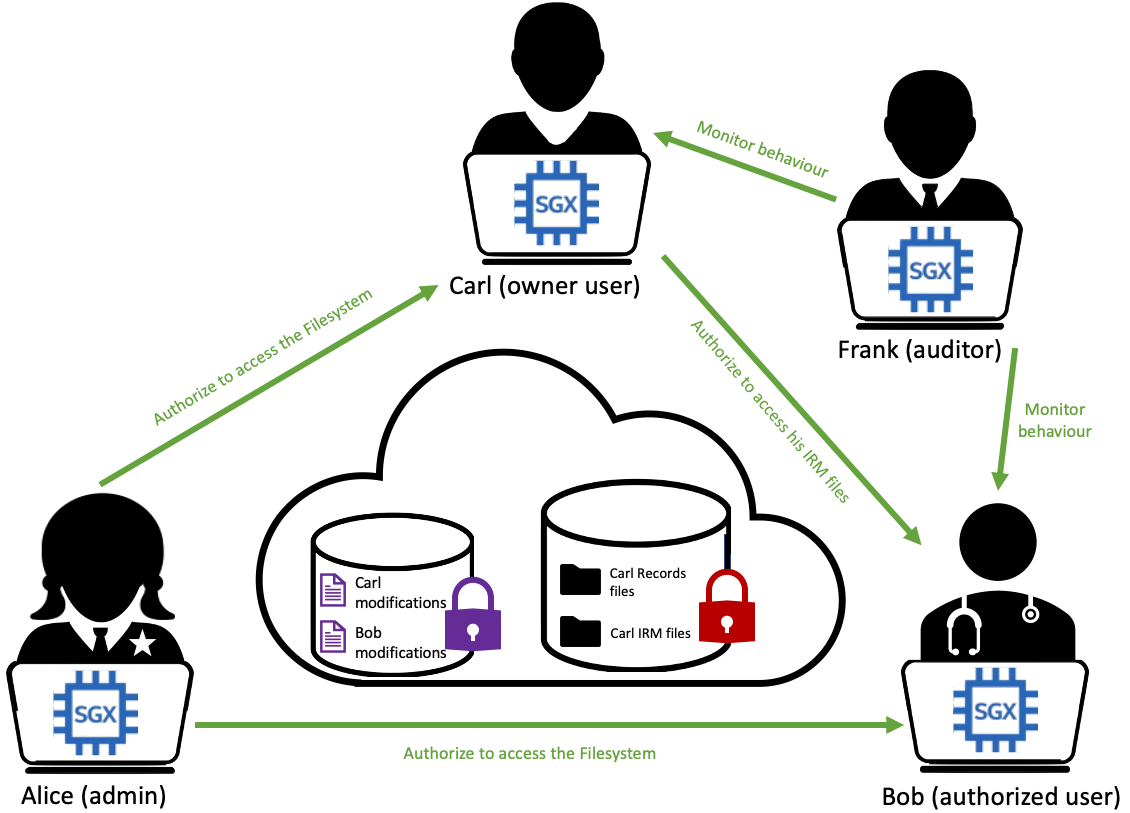
\includegraphics[width=\textwidth]{images/lauxus/approach_trust}
    
    \caption{Trust overview of the protocol to share the FileSystem}
    \label{figure:lauxus:approach_trust}
\end{figure}
\par As presented in the use case Section \ref{section:problem:use_case} the protocol happens between multiple parties (the administrator, the auditor, the owner user and the authorised user). As a quick reminder, all the relations of trust between each of the roles are presented in Figure \ref{figure:lauxus:approach_trust}.

\newpage
\subsection{Filesystem overview}
\label{section:lauxus:approach_fs}
\begin{figure}[h]
    \centering
    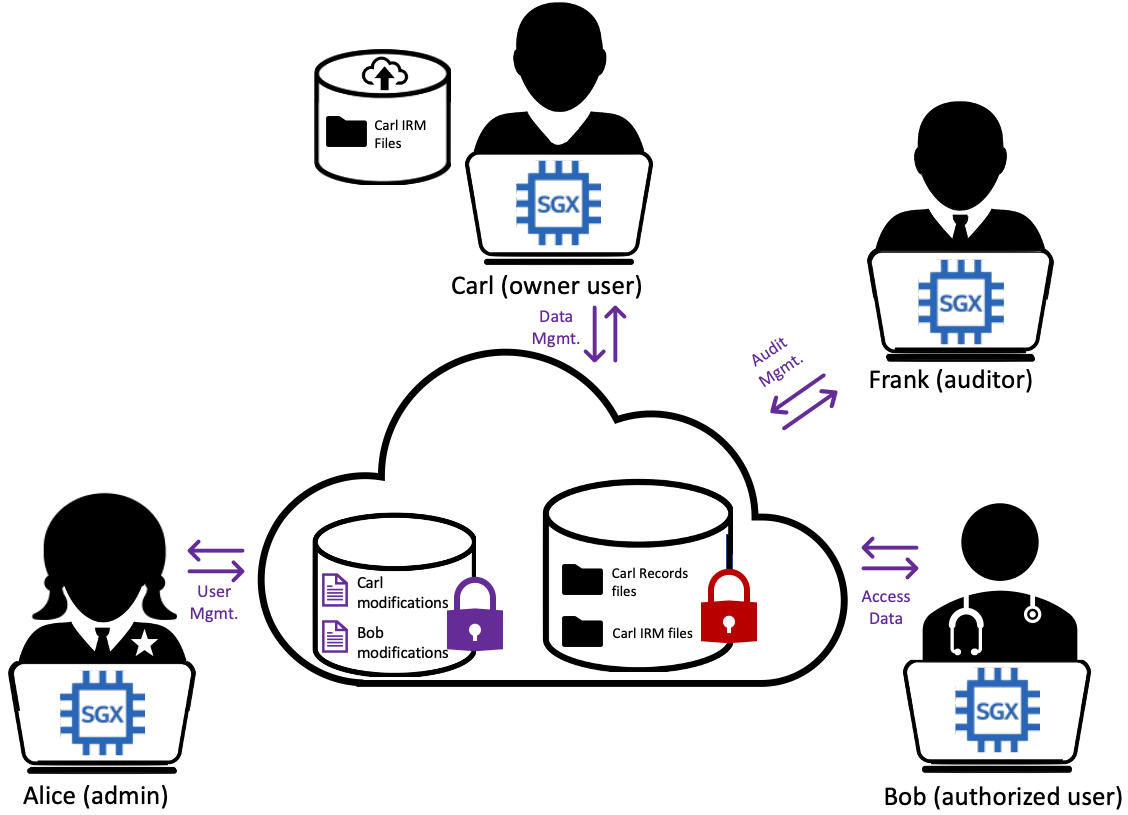
\includegraphics[width=\textwidth]{images/lauxus/approach_fs}
    
    \caption{Filesystem overview of the protocol to share the FileSystem}
    \label{figure:lauxus:approach_fs}
\end{figure}
\par Every user is running \textit{FUSE} to interact with the decrypted Filesystem if they are authorised. The \textit{FUSE} interaction is the core of the untrusted application (happening outside the Enclave). Encrypted information received from \textit{FUSE} is then transmitted inside in the Enclave to be decrypted and processed. In the case of reading a file, \textit{FUSE} sends into the Enclave the encrypted content and the Enclave returns to \textit{FUSE} the decrypted content which is then transmitted to the end-user. The same principle applies upon write operation but in the opposite way: sending decrypted information into the Enclave and outputs the corresponding encrypted information to the remote storage.

\newpage
\subsection{Cryptographic overview}
\label{section:lauxus:approach_crypto}
\begin{figure}[h]
    \centering
    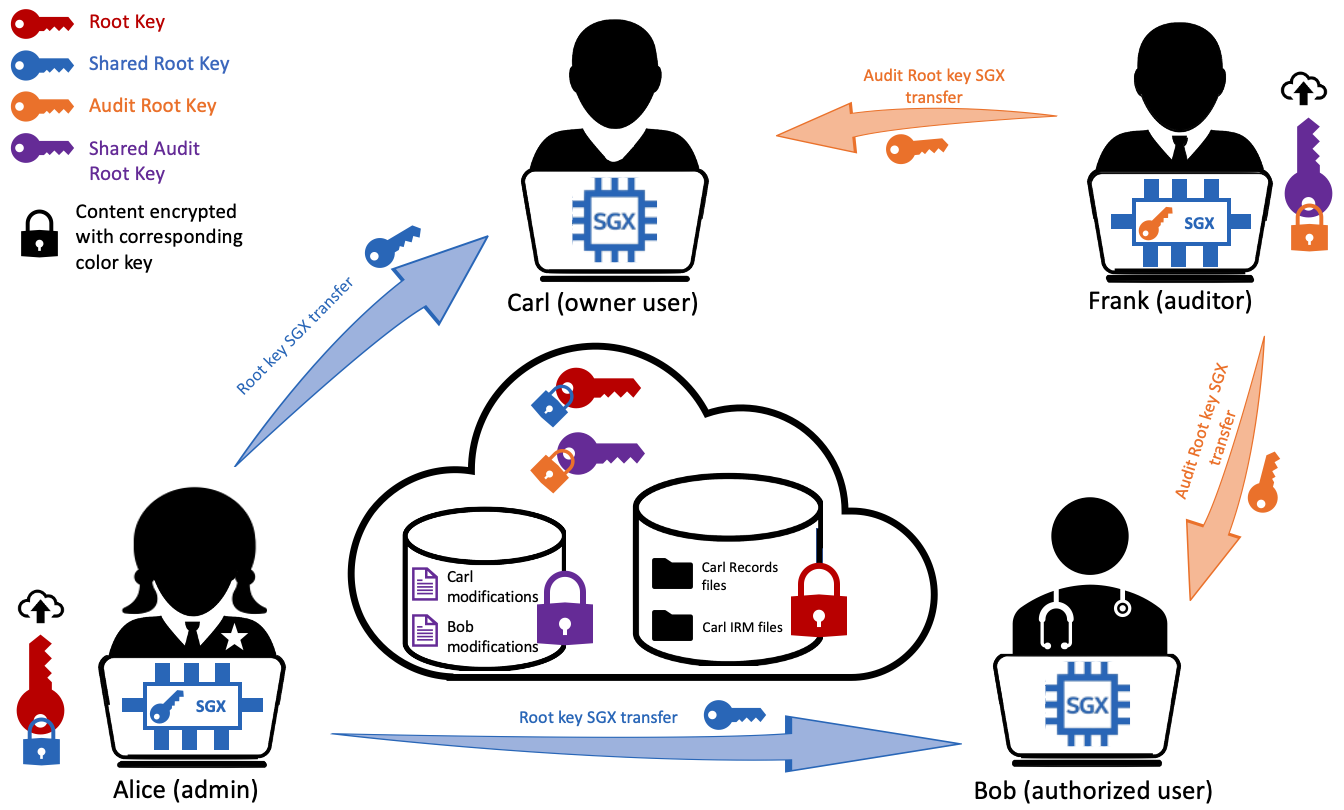
\includegraphics[width=\textwidth]{images/lauxus/approach_crypto}
    
    \caption{Cryptographic overview of the protocol to share the FileSystem}
    \label{figure:lauxus:approach_crypto}
\end{figure}
\par Next, we will take a look at the core of the filesystem, which is its content. To protect confidential information against attackers, the administrator (Alice) will encrypt the filesystem with a secret key (the root key, in red). Then she will upload the encrypted filesystem to the remote storage. To avoid sharing the root key in clear, she will only share it after encrypting it with another key (the shared root key, in blue). This last key will only be transmitted to authorised users through a secure out-of-band channel. This is where we can see the power of SGX and why we chose it: being able to manipulate a secret on a client's computer without revealing any information on this secret to the client itself. Here, the secret we are talking about is the root key. In this way, the intended user, for example, Carl, can decrypt the key located on the storage and retrieve the root key. Then he can access and decrypt the filesystem. After the root key is securely shared between users, it is securely stored inside the user's computer by leveraging SGX Sealing capabilities.

\subsection{Auditing overview}
\label{section:lauxus:approach_audit}
\par Last, we have the auditing files which stores the justifications for every action done by the authorised users along with more contextual information (e.g: the time, the date, etc). There is a 1-to-1 mapping between the auditing files and the files in the filesystem. In practice, the filesystem will create one entry in the appropriate audit file on each read or write of any user, no matter its role. We are using two different keys to have segregation of duties (the administrator manages \textbf{only} the filesystem and the auditor manages \textbf{only} the audits). The idea is that an organisation, here the hospital, can't at the same time read in plaintext the filesystem content and the auditing files. We don't want an organisation to change the auditing file at their advantage. As audit files are used for GDPR purposes, only a trusted entity should read those, thus owning the audit root key. They work similarly than the filesystem content. Here, the auditor is equivalent to the administrator. Thus, the auditor owns the audit root key (the purple key). The sharing of the audit root key follows the same procedure as with the root key. As explained above, the audit root key must also be securely shared to have a working filesystem.

\newpage
\subsection{Global overview}
\label{section:lauxus:approach_global}
\begin{figure}[h]
    \centering
    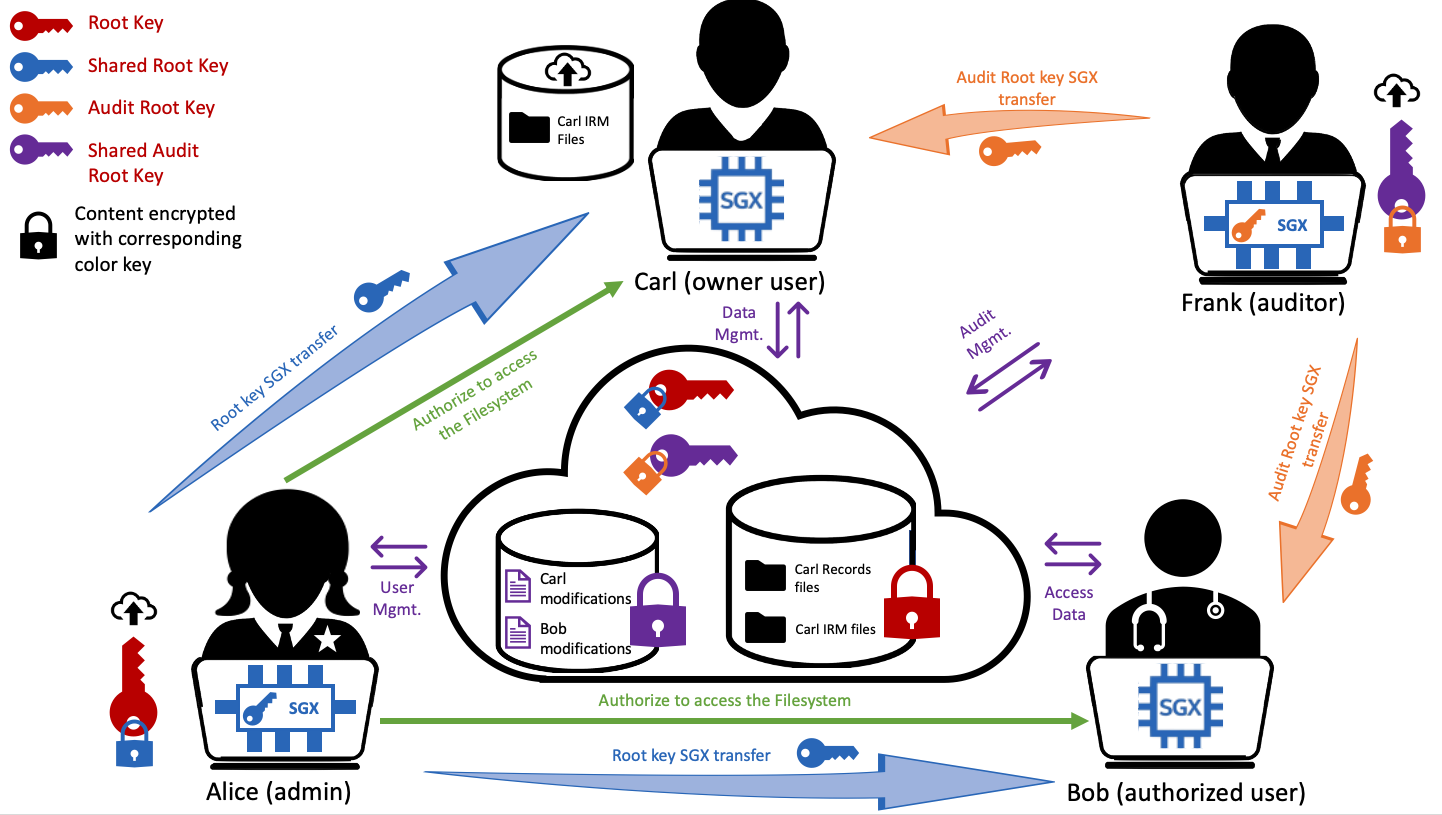
\includegraphics[width=\textwidth]{images/lauxus/approach_global}
    
    \caption{Global overview of the protocol to share the FileSystem}
    \label{figure:lauxus:approach_global}
\end{figure}
\par When we merge all the above-mentionned concepts, we end up with Figure \ref{figure:lauxus:approach_global}. As we can see from the Figure, it is crowded and hard to understand at first sight. Which is why we choose to split it into four parts.
\par An UML state diagram can be found in Appendix \ref{appendix:lauxus_life_state_diagram} for even more detailed information on the whole interaction of the solution.


\end{document} 